
\section{The implementation}


   

    \begin{frame}{Implementation challenges}
    \begin{center}
        This is a great and fun challenge!
    \end{center}
        
        \begin{itemize}
            
            \item How do we decompose the problem to handle the dependency chain?
            \item How do we handle synchronization, shared memory access and cache efficiency?
            \item How do we balance the load?
           
        \end{itemize}
    \end{frame}


    

    \begin{frame}{Our solutions}

        We have experimented 3 different approaches using OpenMP:

        \begin{enumerate}
            \item Using locks
            \item Using atomic counters
            \item Using tasks
        \end{enumerate}
        
    \end{frame}



    \begin{frame}{Locks}
            \begin{minipage}{0.3\linewidth}
           \begin{figure}
           \begin{center}
            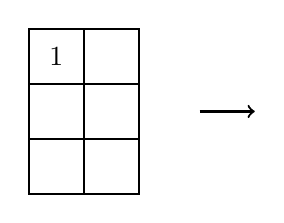
\begin{tikzpicture}[thick,scale=0.7, every node/.style={scale=1}]
                \draw (0,0) -- (0,1) -- (1,1) -- (1,0) -- cycle;
                \draw (1,0) -- (1,1) -- (2,1) -- (2,0) -- cycle;

                \draw (0,1) -- (0,2) -- (1,2) -- (1,1) -- cycle;
                \draw (1,1) -- (1,2) -- (2,2) -- (2,1) -- cycle;

                \draw (0,2) -- (0,3) -- (1,3) -- (1,2) -- cycle;
                \draw (1,2) -- (1,3) -- (2,3) -- (2,2) -- cycle;

                \node at (0.5,2.5) {1};
                \draw[->] (3.1,1.5) -- (4.1, 1.5);
            \end{tikzpicture}
            \end{center}
            \end{figure}
    \end{minipage}
    \hfill
    \begin{minipage}{0.3\linewidth}
           \begin{figure}
           \begin{center}
            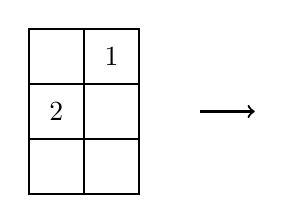
\begin{tikzpicture}[thick,scale=0.7, every node/.style={scale=1}]
                \draw (0,0) -- (0,1) -- (1,1) -- (1,0) -- cycle;
                \draw (1,0) -- (1,1) -- (2,1) -- (2,0) -- cycle;

                \draw (0,1) -- (0,2) -- (1,2) -- (1,1) -- cycle;
                \draw (1,1) -- (1,2) -- (2,2) -- (2,1) -- cycle;

                \draw (0,2) -- (0,3) -- (1,3) -- (1,2) -- cycle;
                \draw (1,2) -- (1,3) -- (2,3) -- (2,2) -- cycle;

                \node at (0.5, 2.5) {\checkmark};
                \node at (1.5,2.5) {1};
                \node at (0.5,1.5) {2};
                \draw[->] (3.1,1.5) -- (4.1, 1.5);
            \end{tikzpicture}
            \end{center}
            \end{figure}
    \end{minipage}
    \hfill
    \begin{minipage}{0.3\linewidth}
           \begin{figure}
           \begin{center}
            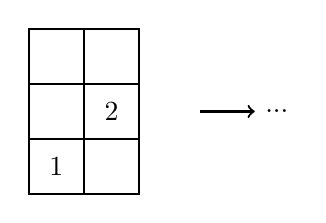
\begin{tikzpicture}[thick,scale=0.7, every node/.style={scale=1}]
                \draw (0,0) -- (0,1) -- (1,1) -- (1,0) -- cycle;
                \draw (1,0) -- (1,1) -- (2,1) -- (2,0) -- cycle;

                \draw (0,1) -- (0,2) -- (1,2) -- (1,1) -- cycle;
                \draw (1,1) -- (1,2) -- (2,2) -- (2,1) -- cycle;

                \draw (0,2) -- (0,3) -- (1,3) -- (1,2) -- cycle;
                \draw (1,2) -- (1,3) -- (2,3) -- (2,2) -- cycle;

                \node at (0.5, 2.5) {\checkmark};
                \node at (1.5, 2.5) {\checkmark};
                \node at (0.5, 1.5) {\checkmark};
                \node at (0.5,0.5) {1};
                \node at (1.5,1.5) {2};
                \draw[->] (3.1,1.5) -- (4.1, 1.5);
                \node at (4.5, 1.5) {...};
            \end{tikzpicture}
            \end{center}
            \end{figure}
    \end{minipage}

        \vspace{10pt}
    
        Divide H in blocks and assign a lock to each. All threads set their own locks.
        
        When a thread wants to work on a block, it sets the lock above it. When it's done, it destroys such lock, and unsets its own. 
    \end{frame}


    \begin{frame}{Atomic counters}

            \begin{minipage}{0.3\linewidth}
           \begin{figure}
           \begin{center}
            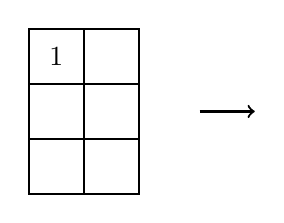
\begin{tikzpicture}[thick,scale=0.7, every node/.style={scale=1}]
                \draw (0,0) -- (0,1) -- (1,1) -- (1,0) -- cycle;
                \draw (1,0) -- (1,1) -- (2,1) -- (2,0) -- cycle;

                \draw (0,1) -- (0,2) -- (1,2) -- (1,1) -- cycle;
                \draw (1,1) -- (1,2) -- (2,2) -- (2,1) -- cycle;

                \draw (0,2) -- (0,3) -- (1,3) -- (1,2) -- cycle;
                \draw (1,2) -- (1,3) -- (2,3) -- (2,2) -- cycle;
                \node at (0.5,2.5) {1};
                \draw[->] (3.1,1.5) -- (4.1, 1.5);
            \end{tikzpicture}
            \end{center}
            \end{figure}
            $C_1 =0, C_2=0$
    \end{minipage}
    \hfill
    \begin{minipage}{0.3\linewidth}
           \begin{figure}
           \begin{center}
            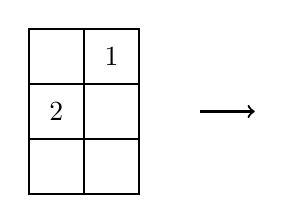
\begin{tikzpicture}[thick,scale=0.7, every node/.style={scale=1}]
                \draw (0,0) -- (0,1) -- (1,1) -- (1,0) -- cycle;
                \draw (1,0) -- (1,1) -- (2,1) -- (2,0) -- cycle;

                \draw (0,1) -- (0,2) -- (1,2) -- (1,1) -- cycle;
                \draw (1,1) -- (1,2) -- (2,2) -- (2,1) -- cycle;

                \draw (0,2) -- (0,3) -- (1,3) -- (1,2) -- cycle;
                \draw (1,2) -- (1,3) -- (2,3) -- (2,2) -- cycle;

                \node at (0.5, 2.5) {\checkmark};
                \node at (1.5,2.5) {1};
                \node at (0.5,1.5) {2};
                \draw[->] (3.1,1.5) -- (4.1, 1.5);
            \end{tikzpicture}
            \end{center}
            \end{figure}
            $C_1 =1, C_2=0$
    \end{minipage}
    \hfill
    \begin{minipage}{0.3\linewidth}
           \begin{figure}
           \begin{center}
            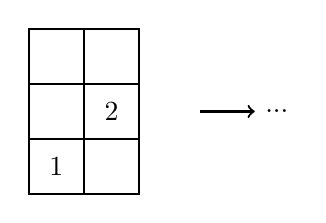
\begin{tikzpicture}[thick,scale=0.7, every node/.style={scale=1}]
                \draw (0,0) -- (0,1) -- (1,1) -- (1,0) -- cycle;
                \draw (1,0) -- (1,1) -- (2,1) -- (2,0) -- cycle;

                \draw (0,1) -- (0,2) -- (1,2) -- (1,1) -- cycle;
                \draw (1,1) -- (1,2) -- (2,2) -- (2,1) -- cycle;

                \draw (0,2) -- (0,3) -- (1,3) -- (1,2) -- cycle;
                \draw (1,2) -- (1,3) -- (2,3) -- (2,2) -- cycle;

               
                \node at (0.5, 2.5) {\checkmark};
                \node at (1.5, 2.5) {\checkmark};
                \node at (0.5, 1.5) {\checkmark};
                \node at (0.5,0.5) {1};
                \node at (1.5,1.5) {2};
                \draw[->] (3.1,1.5) -- (4.1, 1.5);
                \node at (4.5, 1.5) {...};
            \end{tikzpicture}
            \end{center}
            \end{figure}
            $C_1 =2, C_2=1$
    \end{minipage}

        \vspace{10pt}

        Each thread holds a counter of how many blocks it has processed. Thread $i+1$ waits until thread $i$ has processed at least one more block. 

        When threads jump rows the condition is a little different.
        
    \end{frame}



    \begin{frame}{Tasks}
       This is a recursive Divide \& Conquer approach:
       \begin{minipage}{0.55\linewidth}
        \tiny\lstinputlisting{Sections/alg_tasks.cpp}
       \end{minipage}
       \begin{minipage}{0.4\linewidth}
           \begin{figure}
           \begin{center}
            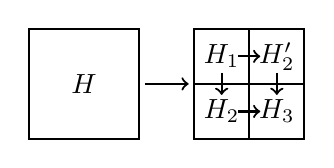
\begin{tikzpicture}[thick,scale=0.7, every node/.style={scale=1}]
                \draw (-1,-1) -- (1,-1) -- (1,1) -- (-1,1) -- cycle;
                \node at (0,0) {$H$};
                \draw[->] (1.1,0) -- (1.9,0);

                \draw (2,0) -- (3,0) -- (3,1) -- (2,1) -- cycle;
                \node at (2.5,+0.5) (A) {$H_1$};
                \draw (2,-1) -- (3,-1) -- (3,0) -- (2,0) -- cycle;
                \node at (2.5,-0.5) (B1) {$H_2$};
                \draw (3,-1) -- (4,-1) -- (4,0) -- (3,0) -- cycle;
                \node at (3.5,+0.5) (B2) {$H_2'$};
                \draw (3,0) -- (4,0) -- (4,1) -- (3,1) -- cycle;
                \node at (3.5,-0.5) (C) {$H_3$};
                \draw[->] (2.5,0.2) -- (2.5,-0.2);
                \draw[->] (2.8,0.5) -- (3.2,0.5);
                %\draw[->] (A) -- (C);
                \draw[->] (3.5,0.2) -- (3.5,-0.2);
                \draw[->] (2.8,-0.5) -- (3.2,-0.5);
            \end{tikzpicture}
            \end{center}
            \end{figure}
        \end{minipage}
    \end{frame}